%%%%%%%%%%%%%%%%%%%%%%%%%%%%%%%%%%%%%%%%%%%%%%%%%%%%%%%%%%%%%%%%%%%%%%%%
%%
%%  Lecture Notes on Computational Astrophysical Hydrodynamics
%%  ICE-SUN Workshop, Kunming, 2024
%%
%%  Originally handwritten August 2024 by R. Fisher.
%%  Transcribed to LaTeX August 3, 2026 by Claude Opus.
%%
%%  NOTE ON PAGE ORDER: the source scan is out of sequence. Handwritten
%%  page 7 continues page 4 (it completes the sentence ending
%%  "...dissipated as heat,"). The logical order followed here is
%%  1, 2, 3, 4, 7, 5, 6, 8, 9, 10, 11, 12, 13.
%%
%%%%%%%%%%%%%%%%%%%%%%%%%%%%%%%%%%%%%%%%%%%%%%%%%%%%%%%%%%%%%%%%%%%%%%%%

\documentclass[notoc]{tufte-handout}
\usepackage{microtype}
\usepackage[utf8]{inputenc}

\usepackage{amsfonts}
\usepackage{amsmath}
\usepackage{amssymb}
\usepackage{physics}
\usepackage{comment}
\usepackage{mathtools}
\usepackage{cancel}

\usepackage{enumerate}
\usepackage{enumitem}

\usepackage{booktabs}
\aboverulesep=0pt
\belowrulesep=0pt

\usepackage{array}
\usepackage{adjustbox}
\usepackage{multicol}

\usepackage{xcolor}
\usepackage{float}

\usepackage{graphicx}
\graphicspath{{../figures/}{./}}
\usepackage{tikz}

%% Live cross-references into the companion handout. Requires
%% hydro_equation_derivation.aux to be present at compile time;
%% build that document first, or references resolve to "??".
\usepackage{xr}
\externaldocument[H-]{hydro_equation_derivation}

\setlength{\headheight}{24pt}
\addtolength{\topmargin}{-9pt}

\newcolumntype{L}[1]{>{\raggedright\arraybackslash}m{#1}}
\newcolumntype{C}[1]{>{\centering\arraybackslash}m{#1}}
\newcolumntype{R}[1]{>{\raggedleft\arraybackslash}m{#1}}

\usepackage{parskip}
\setlength{\parindent}{0pt}
\setlength{\parskip}{1em}


\renewcommand{\vec}[1]{\mathbf{#1}}

\newcommand{\del}{\vec{\nabla}}

\newcommand{\E}{\vec{E}}

\newcommand{\B}{\vec{B}}


\everymath{\displaystyle}

\hypersetup{
  colorlinks = true,
  linkcolor = blue,
  citecolor = blue,
  filecolor = magenta,
  urlcolor = blue,
}

\setcounter{secnumdepth}{2}


\title{Lecture Notes on Computational Astrophysical Hydrodynamics}

\author[Prof. Robert Fisher]{Prof. Robert Fisher\thanks{The University of Massachusetts Dartmouth Department of Physics}\thanks{Heidelberg Institute for Theoretical Studies (HITS), Sabbatical 2023-24}}

\date{ICE-SUN Workshop, Kunming, August 2024.\thanks{Transcribed from handwritten notes to \LaTeX{} on August 3, 2026 by Claude Opus.}}


\begin{document}

\maketitle

\begin{abstract}
These notes accompany a set of introductory lectures on computational astrophysical hydrodynamics. They develop the dimensionless numbers which govern the choice of numerical method in astrophysical flows, the connection between Kolmogorov turbulence and the use of the Euler equations in astrophysics, the finite-volume formulation underlying modern Godunov schemes, and the Taylor-Sedov blastwave as a worked example of a self-similar solution.
\end{abstract}

\newpage

\setcounter{tocdepth}{2}
\tableofcontents

\newpage


\section{Broad Objectives}

\begin{enumerate}
    \item Guided by physical considerations, understand the partial differential equations (PDEs) governing stellar interiors and stellar transients as well as related astrophysical phenomena (such as accretion disks around compact stellar objects).

    \item Understand the numerical methods employed by modern astrophysical codes to solve these PDEs.

    \item Get actual ``hands-on'' experience in doing multidimensional numerical simulations using an open source hydro code (FLASH-X).
\end{enumerate}

While there is an extensive research literature and a growing number of pedagogically-oriented books on computational astrophysics, still today much of the body of knowledge gets passed on ``from master to student.'' An overarching goal of these lectures is to provide some of this less tangible communal knowledge, and a feeling for the choices which must be made by any practicing computational astrophysicist.


\section{Astrophysical Flow Regimes}

No single numerical method is ideally suitable for all astrophysical systems (Fig. \ref{fig:regimes}).

\begin{figure}[htbp]
\centering
\begin{tikzpicture}[scale=0.76]
  % axes
  \draw[->, thick] (0,0) -- (0,4.6);
  \draw[->, thick] (0,0) -- (9.2,0);
  % dividing lines
  \draw[dashed] (0,2.3) -- (9.0,2.3);
  \draw[dashed] (4.3,0) -- (4.3,4.6);
  % axis labels
  \node[rotate=90, anchor=south] at (-0.75,2.3) {\small $\mathrm{Ma} = v/c_s$};
  \node[anchor=east] at (-0.1,3.5) {\small supersonic};
  \node[anchor=east] at (-0.1,1.1) {\small subsonic};
  \node[anchor=east] at (-0.1,2.3) {\small $1$};
  \node[anchor=north] at (2.1,-0.25) {\small short timescales};
  \node[anchor=north] at (7.0,-0.25) {\small long timescales};
  \node[anchor=north] at (9.2,-0.9) {\small $t/t_{\rm dyn}$};
  % quadrant labels
  \node[anchor=north west, align=left] at (0.2,4.4) {\small Compressible Hydro\\[-2pt] \small (FLASH, Athena,\\[-2pt] \small AREPO, etc.)};
  \node[anchor=north west, align=left] at (4.5,4.4) {\small Supersonic Long Duration};
  \node[anchor=north west, align=left] at (0.2,2.1) {\small Low Mach Solvers\\[-2pt] \small (SLH, Maestro, etc.)};
  \node[anchor=north west, align=left] at (4.5,2.1) {\small Stellar evolutionary codes\\[-2pt] \small (MESA, etc.)};
\end{tikzpicture}
\caption{Astrophysical flow regimes. No single numerical method is ideally suitable across the whole plane of Mach number and simulated duration.}
\label{fig:regimes}
\end{figure}
The choice of numerical method depends upon the physical problem and the scales of interest. In astrophysical flows, four numbers largely determine these choices.

\begin{center}
\small
\begin{tabular}{@{}l l@{}}
\toprule
Knudsen number \quad $\mathrm{Kn} = \frac{\lambda_{\rm mf}}{L}$ & mean-free path to typical scale \\
Mach number \quad $\mathrm{Ma} = \frac{v}{c_s}$ & flow to sound speed \\
Reynolds number \quad $\mathrm{Re} = \frac{L v}{\nu}$ & inertial to viscous forces \\
Plasma parameter \quad $\beta = \frac{P_g}{P_m}$ & gas to magnetic pressure \\
\bottomrule
\end{tabular}
\end{center}

We examine each of these in turn.

\subsection{Knudsen Number \texorpdfstring{$\mathrm{Kn}$}{Kn}}

The Knudsen number is one of the most basic parameters which qualitatively determines the character of the flow. If $\mathrm{Kn} \ll 1$, the mean-free path length is much smaller than length scales of interest, and the fluid flow can therefore be treated as a continuum, with all fluid quantities (mass density, temperature, etc.) smoothly defined (outside of shocks). \marginnote{Recall that $\lambda_{\rm mf} \, \sigma \, n \sim 1$, so that $\lambda_{\rm mf} \sim 1 / (n\sigma)$, with $\sigma$ the collisional cross section.}

Conversely, if $\mathrm{Kn} \gtrsim 1$, the fluid flow cannot be represented as a continuous medium, typically requiring the material particles (ions and electrons) to be treated by more fundamental physical descriptions of plasma physics.

\subsection{Estimating the Mean-Free Path in an Ionized Plasma}

Estimate a large deflection when\footnote{Small angle deflections are typically more important, and bring in a factor of the inverse of the Coulomb logarithm parameter --- see Shu, v. II, chapter I.}

\begin{equation}
\frac{e^2}{r_{\rm eff}} \sim m_e w^2 \sim k T_e
\end{equation}
%
where $w$ is the relative velocity and $r_{\rm eff}$ is the effective impact parameter at which a large-angle deflection occurs (Fig. \ref{fig:scattering}).

\begin{figure}[htbp]
\centering
\begin{tikzpicture}[scale=1.0]
  % upper electron: enters from lower left, deflects up and to the right
  \draw[thick, ->] (0.1,1.55) .. controls (1.9,1.55) and (2.7,1.72) .. (4.9,2.5);
  \node[anchor=south east] at (0.35,1.55) {\small $e^-$};
  % lower electron: enters from upper right, deflects down and to the left
  \draw[thick, ->] (4.9,0.55) .. controls (2.7,0.55) and (1.9,0.72) .. (0.1,-0.25);
  \node[anchor=south west] at (4.65,0.55) {\small $e^-$};
  % impact parameter
  \draw[<->] (3.05,0.62) -- (3.05,1.72);
  \node[anchor=west] at (3.15,1.17) {\small $r_{\rm eff}$};
\end{tikzpicture}
\caption{Coulomb scattering of two electrons. A large-angle deflection occurs when the impact parameter falls to $r_{\rm eff}$, where the electrostatic potential energy is comparable to the thermal energy.}
\label{fig:scattering}
\end{figure}

Then

\begin{equation}
\lambda_{\rm mf} \sim \frac{1}{n_e \sigma} \sim \frac{1}{n_e \pi r_{\rm eff}^2} \sim \frac{\left( k T_e \right)^2}{n_e e^4}
\end{equation}

For the sun, $n_e \approx \rho / m_u$, assuming $X \approx 1$. At the center of the sun ($T \sim 10^7$ K, $\rho \sim 100$ g/cm$^3$):

\begin{equation}
\lambda_{\rm mf} \sim \frac{\left( k T_e \right)^2 m_u}{\rho \, e^4} \sim 50 \times 10^{-8}~\text{cm}
\end{equation}

This length scale is enormously smaller than the radius or pressure scale height of the stellar interior

\begin{equation}
\mathrm{Kn} = \frac{\lambda_{\rm mf}}{R_\odot} \sim \frac{50 \times 10^{-8}~\text{cm}}{7 \times 10^{10}~\text{cm}} \sim 7 \times 10^{-18}
\end{equation}

The small $\mathrm{Kn}$ number also implies collision times between charged species are so short that all species will relax to Maxwellian on times

\begin{equation}
t_c \sim \frac{\lambda_{\rm mf}}{v} \sim \frac{\lambda_{\rm mf} \, m_e^{1/2}}{\left( k T_e \right)^{1/2}} \sim 10 \times 10^{-17}~\text{s}
\end{equation}

Which implies that electrons and ions have a single shared temperature, and that a local thermodynamic approximation applies throughout the stellar interior.

\subsection{Mach Number \texorpdfstring{$\mathrm{Ma}$}{Ma}}

The Mach number determines the degree of compressibility of the fluid.


\section{Kolmogorov Turbulence and the Reynolds Number}

Assume a self-similar steady cascade from the large scale $\sim L$ (the integral scale), down to the smallest length scale $\eta$, which is called the Kolmogorov scale (Fig. \ref{fig:spectrum}). Further, call $\delta v_L \equiv v_0$.

\begin{figure}[htbp]
\centering
\begin{tikzpicture}[scale=0.95]
  \draw[->, thick] (0,0) -- (0,3.5) node[anchor=south east] {\small $E(k)$};
  \draw[->, thick] (0,0) -- (7.7,0) node[anchor=north east] {\small $k$};
  % rise to the driving peak
  \draw[thick] (0.30,0.15) .. controls (0.60,1.30) and (0.72,2.60) .. (0.90,2.90);
  % inertial range through the dissipation cutoff: strictly positive
  \draw[thick, domain=0.90:6.95, samples=120, smooth]
        plot (\x, {2.90*exp(-0.22*(\x-0.9) - 0.010*(\x-0.9)*(\x-0.9)*(\x-0.9))});
  \draw[dashed] (0.90,0) -- (0.90,2.90);
  \draw[dashed] (6.20,0) -- (6.20,0.21);
  \node[anchor=south] at (0.90,2.97) {\small $k \sim 1/L$};
  \node[anchor=south west] at (6.05,0.30) {\small $k \sim 1/\eta$};
  \node[anchor=north] at (0.55,-0.62) {\small driving};
  \node[anchor=north] at (3.55,-0.62) {\small inertial range};
  \node[anchor=north] at (7.05,-0.62) {\small dissipation};
  \draw[<->] (1.00,-0.45) -- (6.10,-0.45);
  \draw[dotted] (0.90,-0.30) -- (0.90,-0.60);
  \draw[dotted] (6.20,-0.30) -- (6.20,-0.60);
\end{tikzpicture}
\caption{The turbulent energy spectrum $E(k)$, showing the driving scale $k \sim 1/L$, the inertial range over which the Kolmogorov cascade operates, and the dissipation cutoff at the Kolmogorov scale $k \sim 1/\eta$.}
\label{fig:spectrum}
\end{figure}

Write $\delta v_r$ for the velocity fluctuation on scale $r$, so that the eddy turnover time on that scale is \marginnote{These concepts can be made more rigorous by Fourier transforming the specific kinetic energy $v^2$ from real to Fourier space.}

\begin{equation}
t_{\rm eddy}(r) = \frac{r}{\delta v_r}
\end{equation}

For steady turbulence, the flux of kinetic energy is the same on all scales $r < L$:

\begin{equation}
\text{rate of spec. KE per time} \quad = \quad \frac{v_0^2}{\left( L / v_0 \right)} \quad = \quad \frac{\delta v_r^2}{\left( r / \delta v_r \right)}
\end{equation}

\begin{equation}
\frac{v_0^3}{L} = \frac{\delta v_r^3}{r}
\end{equation}
%
This carries all the way down to $r \sim \eta$, where turbulence is dissipated. Rearranging,

\begin{equation}
\boxed{ \delta v_r = v_0 \left( \frac{r}{L} \right)^{1/3} }
\end{equation}
%
which is the Kolmogorov velocity scaling. This rate of turbulent energy dissipation is written as $\varepsilon = v_0^3 / L$ and is an invariant constant quantity for steady driven turbulence with fixed $v_0$ and $L$.

But this cannot extend to arbitrarily short length scales. When $t_{\rm eddy}(\eta) \sim t_{\rm visc}(\eta)$, the eddy cannot turn over before it is dissipated as heat,

\begin{equation}
\eta = \left( \frac{\nu^3}{\varepsilon} \right)^{1/4}
\end{equation}
%
which is the Kolmogorov length scale. The ratio of the large-scale integral driving length scale, down to the smallest Kolmogorov length scale is

\begin{align}
\frac{L}{\eta} & = \frac{L \, \varepsilon^{1/4}}{\nu^{3/4}} = \frac{L \, v_0^{3/4}}{\nu^{3/4} L^{1/4}} \\
& = \left( \frac{L v_0}{\nu} \right)^{3/4} = \mathrm{Re}^{3/4}
\label{eqn:Rescaling}
\end{align}

The Reynolds number is normally introduced as the ratio of the importance of inertial to viscous forces

\begin{equation}
\frac{\partial (\rho v_i)}{\partial t} + \sum_j \left( \frac{\partial \Pi_{ij}}{\partial x_j} + \frac{\partial S_{ij}}{\partial x_j} \right) = 0
\label{eqn:reynolds_momentum}
\end{equation}
%
for zero net force, where $S_{ij}$ is the viscous stress tensor,

\begin{equation}
S_{ij} = \rho \nu \left( \underbrace{\frac{\partial v_i}{\partial x_j} + \frac{\partial v_j}{\partial x_i}}_{\text{deformation}} - \underbrace{\frac{2}{3}\delta_{ij}\frac{\partial v_k}{\partial x_k}}_{\text{dilation}} \right)
\end{equation}

Equation \ref{eqn:reynolds_momentum} is the momentum equation derived in the companion notes,\footnote{{\it The Fundamental Equations of Hydrodynamics and Ideal Magnetohydrodynamics for Astrophysical Flows}, \S 1.2.} Equation \ref{H-eqn:momentum_equation} there, with the body force switched off and a viscous stress restored alongside the ideal momentum flux. The tensor $\Pi_{ij} = p\,\delta_{ij} + \rho v_i v_j$ is the same object in both. $S_{ij}$ carries exactly the physics which the {\it ideal} stress tensor $\sigma_{ij} = -p\,\delta_{ij}$ of that discussion discards, with the dynamic and kinematic viscosities related by $\mu = \rho\nu$.

\begin{equation}
\text{Ratio} = \frac{\Pi_{ij}}{S_{ij}} \sim \frac{\rho v_0^2}{\rho \nu v_0 / L} \sim \frac{L v_0}{\nu}
\end{equation}
%
In this interpretation, a high Reynolds number flow is one where viscous forces are very weak compared to inertial forces due to pressure.

The one exception arises on very small scales, comparable to the mean free path $\lambda_{\rm mf}$ of the gas particles in the system --- precisely the scales we estimated in \S 2.2. Perhaps the most notable such exception is the shock front itself, whose interior requires viscous forces to ultimately mediate the conversion of bulk kinetic energy into heat. Modern numerical methods, however, effectively sidestep this problem, because the conservation of mass, momentum, and energy alone suffice to determine the strength of the shock front. This is the deeper reason for insisting upon the conservative formulation we develop in \S 4: a scheme which conserves the right quantities will place a shock at the right speed and with the right jump across it, whether or not it resolves anything whatsoever about the interior of the front.

But turbulence provides us with another way to think about the Reynolds number --- as simply the dynamic range (to the $4/3$ power) between the largest and smallest scales of turbulence.

\begin{equation}
\boxed{ \mathrm{Re} = \left( \frac{L}{\eta} \right)^{4/3} }
\end{equation}

\subsection{Kolmogorov Turbulence and the Euler Equations}

Most astrophysical flows have exceedingly high Reynolds numbers --- for example, flows $v_0 \sim 10$ km/s, $L \sim 10^2$ km, inside WDs have $\mathrm{Re} \sim 10^{16}$. Fundamentally, this is because there exists an enormous dynamic range between the scales $\sim L$ where we examine the flow and the Kolmogorov scale where turbulence is dissipated.

{\bf If} the physical viscosity were to be employed in a full Navier-Stokes simulation of these flows, its effect would be negligible.

\begin{center}
\fbox{
\begin{minipage}{0.86\linewidth}
\centering
Physical viscosity (almost!) never matters in astrophysics.
\end{minipage}
}
\end{center}

The reason why can again be understood from the $\mathrm{Re}^{3/4} = L / \eta$ scaling of Equation \ref{eqn:Rescaling}. To imply we are simulating a $\mathrm{Re} = 10^{16}$ flow means we would need $\eta = 10^{-12} L$! Clearly, no simulation completed to date even approaches this value. Instead, the record-holding simulations have of order $\left( 10^4 \right)^3$ cells, implying $\mathrm{Re} \sim 10^5$, effectively.

What is happening inside the simulation is that the grid effectively dissipates kinetic energy on the grid scale $\Delta$ and acts as an effective viscosity with $\eta \sim \Delta$. \marginnote{Momentum conservation of flows into a cell produces heating: two oppositely-directed momentum fluxes $(\rho \vec{v})_1$ and $(\rho \vec{v})_2$ entering a cell cancel in momentum but deposit their kinetic energy as internal energy $\rho \epsilon_{\rm int}$.}

Because the effective Reynolds number is almost always much smaller than the physical Reynolds number, we employ the Euler equations of inviscid hydrodynamics,

\begin{align}
\frac{\partial \rho}{\partial t} + \del\cdot(\rho\vec{v}) & = 0 \\
\frac{\partial (\rho v_i)}{\partial t} + \sum_j \frac{\partial \Pi_{ij}}{\partial x_j} & = F_{v,i} \\
\frac{\partial (\rho E)}{\partial t} + \sum_i \frac{\partial \left[ (\rho E + p) v_i \right]}{\partial x_i} & = \sum_i F_{v,i} v_i
\end{align}
%
with body force $F_{v,i}$, momentum flux tensor $\Pi_{ij} = p \, \delta_{ij} + \rho v_i v_j$, body work $\sum_i F_{v,i}v_i$, and specific total energy $E = \epsilon_{\rm int} + \frac{1}{2}v^2$.

There is no physical viscosity in these equations, but the numerical simulations possess {\it numerical} viscosity as described above, or {\it artificial} viscosity (usually very small in modern numerical methods) introduced ``by hand.'' This is an extremely important point about simulating hydrodynamical flows, even though it is extremely challenging to accurately characterize the precise level of viscosity introduced (see Benzi, Biferale, Fisher et al., PRL {\bf 100}, 234503).


\section{Numerical Solutions of Conservation Law Systems}

Consider the model system of advection of a scalar field $\varphi$ in the presence of a fixed uniform background velocity $\vec{v}$,

\begin{equation}
\frac{\partial \varphi}{\partial t} + \del\cdot\vec{f} = 0, \qquad \vec{f} = \varphi \vec{v}
\end{equation}
%
where $\vec{f}$ is the flux vector. This equation would for example apply to the mass density $\rho$ in hydrodynamics, with a fixed velocity field $\vec{v}$, and many other examples besides (eg, composition in non-reacting flows).

To solve this equation, let's take the simplified case of a 1D flow with constant background velocity, $\vec{v} = (v_x, 0, 0)$. Let's also assume the spatial and time discretization is uniform (all of those assumptions can, of course, be relaxed in more general schemes).

\begin{figure}[htbp]
\centering
\begin{tikzpicture}[scale=1.0]
  \draw[->, thick] (0,0) -- (7.2,0) node[anchor=north] {\small $x$};
  \draw[->, thick] (0,0) -- (0,3.4) node[anchor=east] {\small $t$};
  % control volume
  \draw[thick] (3.0,1.0) rectangle (5.0,2.6);
  % ticks
  \draw (3.0,-0.1) -- (3.0,0.1);
  \draw (4.0,-0.1) -- (4.0,0.1);
  \draw (5.0,-0.1) -- (5.0,0.1);
  \node[anchor=north] at (3.0,-0.15) {\small $x_{i-1/2}$};
  \node[anchor=north] at (4.0,-0.15) {\small $x_i$};
  \node[anchor=north] at (5.0,-0.15) {\small $x_{i+1/2}$};
  \draw (-0.1,1.0) -- (0.1,1.0);
  \draw (-0.1,2.6) -- (0.1,2.6);
  \node[anchor=east] at (-0.15,1.0) {\small $t_n$};
  \node[anchor=east] at (-0.15,2.6) {\small $t_{n+1}$};
  % dimension arrows
  \draw[<->] (3.0,2.95) -- (5.0,2.95) node[midway, above] {\small $\Delta x$};
  \draw[<->] (5.7,1.0) -- (5.7,2.6) node[midway, right] {\small $\Delta t$};
\end{tikzpicture}
\caption{The space-time control volume over which the conservation law is integrated, of width $\Delta x$ and height $\Delta t$.}
\label{fig:controlvolume}
\end{figure}

Integrate the scalar field conservation equation over the control volume of Fig. \ref{fig:controlvolume}, first in space --- from $x_{i-1/2}$ to $x_{i+1/2}$:

\begin{equation}
\int_{x_{i-1/2}}^{x_{i+1/2}} \frac{\partial \varphi}{\partial t}~\mathrm{d}x + \int_{x_{i-1/2}}^{x_{i+1/2}} \frac{\partial f}{\partial x}~\mathrm{d}x = 0
\end{equation}

\begin{equation}
\int_{x_{i-1/2}}^{x_{i+1/2}} \frac{\partial \varphi}{\partial t}~\mathrm{d}x + \left[ f(x_{i+1/2}) - f(x_{i-1/2}) \right] = 0
\end{equation}

Next, integrate this result in time from $t_n$ to $t_{n+1}$:

\begin{equation}
\int_{t_n}^{t_{n+1}}\int_{x_{i-1/2}}^{x_{i+1/2}} \frac{\partial \varphi}{\partial t}~\mathrm{d}x\,\mathrm{d}t + \int_{t_n}^{t_{n+1}} \left[ f(x_{i+1/2}) - f(x_{i-1/2}) \right]~\mathrm{d}t = 0
\end{equation}

Assuming the integrand $\partial \varphi / \partial t$ is continuous, the order of integration in the first integral can be exchanged:

\begin{equation}
\int_{x_{i-1/2}}^{x_{i+1/2}}\int_{t_n}^{t_{n+1}} \frac{\partial \varphi}{\partial t}~\mathrm{d}t\,\mathrm{d}x + \int_{t_n}^{t_{n+1}} \left[ f(x_{i+1/2}) - f(x_{i-1/2}) \right]~\mathrm{d}t = 0
\end{equation}

\begin{equation}
\hypertarget{star}{}\begin{split}
\int_{x_{i-1/2}}^{x_{i+1/2}} \left[ \varphi(x,t_{n+1}) - \varphi(x,t_n) \right]\mathrm{d}x & \\
+ \int_{t_n}^{t_{n+1}} \left[ f(x_{i+1/2}) - f(x_{i-1/2}) \right]~\mathrm{d}t & = 0 \qquad (*)
\end{split}
\label{eqn:exact}
\end{equation}

The first term can be cast in a more familiar form by expressing it in terms of the spatial average over the cell width $\Delta x$

\begin{equation}
\bar{\varphi}(t) = \frac{1}{\Delta x}\int_{x_{i-1/2}}^{x_{i+1/2}} \varphi(x,t)~\mathrm{d}x
\end{equation}

So $(*)$ becomes

\begin{equation}
\Delta x \left[ \bar{\varphi}(t_{n+1}) - \bar{\varphi}(t_n) \right] + \int_{t_n}^{t_{n+1}} \left[ f(x_{i+1/2}) - f(x_{i-1/2}) \right]~\mathrm{d}t = 0
\end{equation}

This equation is so far {\bf exact}, and has a very simple interpretation --- the update to the conserved scalar field is simply determined by the time-integrated fluxes around the boundaries of cells.

\begin{equation}
\bar{\varphi}(t_{n+1}) = \bar{\varphi}(t_n) - \frac{1}{\Delta x}\int_{t_n}^{t_{n+1}} \left[ f(x_{i+1/2}) - f(x_{i-1/2}) \right]~\mathrm{d}t
\end{equation}

The values of $\varphi$ are naturally ``cell-centered'' in this approach --- meaning the values stored at $\varphi(t_n)$ are naturally the spatial averaged quantities in each cell. One more step represents the fluxes as time-averages,

\begin{equation}
\bar{f}(x_{i-1/2}) = \frac{1}{\Delta t}\int_{t_n}^{t_{n+1}} f(x_{i-1/2})~\mathrm{d}t
\label{eqn:tavgflux}
\end{equation}

So that the entire problem boils down to obtaining the time-averaged fluxes $\bar{f}(x_{i-1/2})$, etc. around cell interfaces and applying these to the conservative update through

\begin{equation}
\boxed{ \bar{\varphi}(t_{n+1}) = \bar{\varphi}(t_n) - \frac{\Delta t}{\Delta x}\left[ \bar{f}(x_{i+1/2}) - \bar{f}(x_{i-1/2}) \right] }
\label{eqn:update}
\end{equation}

\subsection{Finite Difference versus Godunov Methods}

Finite difference methods apply discretized stencils typically directly to the beginning PDEs. In supersonic flows, strong shocks lead to discontinuities where the discretization leads to problematic oscillations around the shock fronts (also contact discontinuities) --- the ``Gibbs phenomenon'' (Fig. \ref{fig:gibbs}).

\begin{figure}[htbp]
\centering
\begin{tikzpicture}[scale=1.0]
  \draw[->, thick] (0,0) -- (5.4,0) node[anchor=north] {\small $x$};
  \draw[->, thick] (0,0) -- (0,3.0) node[anchor=east] {\small $\rho$};
  \draw[thick] (0.3,0.6) -- (2.0,0.6);
  % oscillations before jump
  \draw[thick] (2.0,0.6) .. controls (2.15,1.1) and (2.25,0.3) .. (2.4,0.75);
  \draw[thick] (2.4,0.75) -- (2.55,2.3);
  \draw[thick] (2.55,2.3) .. controls (2.7,2.75) and (2.85,2.05) .. (3.0,2.45);
  \draw[thick] (3.0,2.45) -- (3.15,2.45);
  \draw[thick] (3.15,2.45) -- (3.3,0.75);
  \draw[thick] (3.3,0.75) .. controls (3.45,0.35) and (3.6,0.95) .. (3.75,0.6);
  \draw[thick] (3.75,0.6) -- (5.0,0.6);
  \draw[->] (4.05,2.75) -- (2.72,2.55);
  \node[anchor=west, align=left] at (4.0,2.7) {\small ``Gibbs\\[-2pt] \small phenomenon''};
\end{tikzpicture}
\caption{Spurious oscillations around a strong shock front produced by a finite difference discretization, the ``Gibbs phenomenon.''}
\label{fig:gibbs}
\end{figure}

Alternatively, Godunov methods, which underly most modern astrophysical grid and mesh codes (and even smoothed particle hydrodynamics codes) employ a clever conception of the cell data which does not presume the smoothness of the underlying flow (Fig. \ref{fig:godunov}).

\begin{figure}[htbp]
\centering
\begin{tikzpicture}[scale=0.95]
  % two time levels joined by the cell interface
  \draw[thick] (0.6,0) -- (6.2,0);
  \draw[thick] (0.6,1.9) -- (6.2,1.9);
  \draw[thick] (3.4,0) -- (3.4,1.9);
  \fill (2.0,0) circle (1.6pt);
  \fill (4.8,0) circle (1.6pt);
  \node[anchor=north] at (2.0,-0.1) {\small $x_{i-1}$};
  \node[anchor=north] at (4.8,-0.1) {\small $x_i$};
  \node[anchor=east] at (0.5,0) {\small $t_n$};
  \node[anchor=east] at (0.5,1.9) {\small $t_{n+1}$};
  \node[anchor=south] at (3.4,2.0) {\small $x_{i-1/2}$ interface};
  \draw[->] (5.3,1.0) -- (3.5,0.95);
  \node[anchor=west, align=left] at (5.25,1.0) {\small need to find\\[-2pt] \small time-averaged\\[-2pt] \small flux here};
\end{tikzpicture}
\caption{The Godunov conception of the cell data. The initial data are treated as discontinuous across the $x_{i-1/2}$ interface, and the Riemann problem is solved to obtain the time-averaged flux there.}
\label{fig:godunov}
\end{figure}

The Riemann problem addresses this problem, treating the initial data as discontinuous, and asking what the solution along the interface is.

\subsection{Godunov's Theorem}

The scheme described above turns out to only be first-order accurate in both space and time --- that is, the errors diminish with $\mathcal{O}(\Delta x)$. Godunov's theorem proves that (in 1959) linear schemes which preserve monotonicity (eg, if $\varphi_n(x)$ is monotonically increasing or decreasing in $x$, so too is $\varphi_{n+1}(x)$) are necessarily only first-order accurate. This may seem to be a roadblock to developing higher-order accuracy schemes, but the solution (which took 20+ years to fully develop) is to utilize nonlinear reconstruction slopes and slope limiters on the initial data at $t_n$. This is the basis of the PPM and many other methods.


\subsection{A First-Order Godunov Scheme for Scalar Advection}

Let's assemble these ideas into the simplest complete scheme, for the scalar advection problem we began with. The conservative update, Equation \ref{eqn:update}, is exact, and asks of us only the time-averaged fluxes at the cell interfaces. A Godunov scheme obtains those fluxes through a three-stage cycle, repeated every timestep: \marginnote{From here on we write $\bar{\varphi}_i^{\,n}$ for the average of $\varphi$ over cell $i$ at time $t_n$, which is less cumbersome than $\bar{\varphi}(t_n)$ once several cells are in play at once.}

\begin{enumerate}
    \item {\bf Reconstruct.} From the cell averages $\bar{\varphi}_i^{\,n}$, build a piecewise polynomial representation of $\varphi(x)$ within each cell.
    \item {\bf Solve.} At each interface, solve the Riemann problem posed by the two reconstructed states which meet there, and from its solution obtain the interface flux. This is the {\it corrector} step.
    \item {\bf Update.} Apply the conservative update, Equation \ref{eqn:update}, to advance the cell averages to $t_{n+1}$.
\end{enumerate}

The first-order scheme makes the simplest possible choice at the first stage: the reconstruction is piecewise {\it constant},

\begin{equation}
\varphi(x, t_n) = \bar{\varphi}_i^{\,n}, \qquad x_{i-1/2} < x < x_{i+1/2}
\end{equation}
%
This is the only choice which requires no information whatsoever beyond the cell average itself, and it is exactly the picture sketched in Fig. \ref{fig:godunov}. Its immediate consequence is that the reconstructed data are discontinuous at every cell interface --- and this is a feature rather than a defect. We are not going to smooth over the jump. We are going to solve for the evolution of the jump exactly.

\subsection{The Riemann Problem and the Corrector Step}

Before writing anything down, it is worth having a physical picture in hand, because the name makes this sound far more forbidding than it is.

Imagine a long tube divided in half by a thin diaphragm. On the left is gas in one uniform state --- some density, some pressure, perhaps drifting along at some velocity --- and on the right is gas in a different uniform state. Nothing varies within either half. All of the structure in the problem sits in the single jump at the diaphragm. Now burst the diaphragm. {\it What happens next?} That question, and nothing more, is the Riemann problem.

For a real gas the answer is rich. A shock runs one way, a rarefaction fan spreads the other, and a contact discontinuity drifts between them, separating the material which was originally on the left from the material which was originally on the right. This is the shock tube of the laboratory, and it is the first test problem run on essentially every hydrodynamics code ever written. \marginnote{The standard version, with a particular choice of left and right states, is due to Sod (1978). If you write a hydrodynamics code, this is the problem you will run first, and it is the problem that will tell you what you got wrong.}

Now notice what the piecewise constant reconstruction of \S 4.3 has quietly done. By insisting that $\varphi$ take a single value throughout each cell, we have built ourselves a wall of diaphragms --- one at every cell interface --- and a timestep amounts to bursting all of them at once and asking how far the resulting waves travel before we next look. That is the whole of the Godunov idea. We cannot solve the equations exactly across the entire grid, but we can solve this one small problem exactly, over and over, at every interface, and stitch the answers together with a conservative update.

Our case is the gentlest possible version of it. There is no pressure and no sound speed here, so nothing runs either way --- there is only a scalar being carried downstream at a fixed velocity. Think of dye in a pipe of flowing water, a lighter concentration upstream of a darker one. Burst the diaphragm and nothing dramatic happens at all: the boundary between the two simply drifts along with the water.

At the interface $x_{i-1/2}$, the reconstructed data pose the initial value problem

\begin{equation}
\frac{\partial \varphi}{\partial t} + v_x \frac{\partial \varphi}{\partial x} = 0, \qquad
\varphi(x,t_n) = \begin{cases}
\varphi_L \equiv \bar{\varphi}_{i-1}^{\,n}, & x < x_{i-1/2} \\
\varphi_R \equiv \bar{\varphi}_{i}^{\,n}, & x > x_{i-1/2}
\end{cases}
\end{equation}
%
This is the {\it Riemann problem}: a conservation law together with two constant states separated by a single discontinuity. For linear advection its solution is immediate, since the initial profile is simply translated at the constant speed $v_x$,

\begin{equation}
\varphi(x,t) = \varphi\left(x - v_x (t - t_n),\, t_n \right)
\end{equation}
%
so that the discontinuity propagates along the characteristic $x = x_{i-1/2} + v_x (t-t_n)$, as sketched in Fig. \ref{fig:riemann}.

It is worth pausing on the structure of this solution, because it is what makes the whole scheme practical. The Riemann problem possesses no intrinsic length or time scale --- it is built from nothing but two constant states and a scale-free equation --- and so, exactly as with the blastwave of \S 5, its solution can only be {\it self-similar}. It depends upon $x$ and $t$ solely through the combination \marginnote{Here, and in Fig. \ref{fig:riemann}, $x$ and $t$ are measured from the origin of the Riemann problem itself, at the interface $x_{i-1/2}$ and the time $t_n$.}

\begin{equation}
\frac{x}{t} ~\longrightarrow~ \frac{x - x_{i-1/2}}{t - t_n}
\end{equation}
%
and not upon $x$ and $t$ separately. Every ray of constant $x/t$ drawn out of that origin therefore carries a single constant value of $\varphi$. The discontinuity itself rides the ray $x/t = v_x$, while the flux we require sits on the ray $x/t = 0$ --- the vertical dashed line in Fig. \ref{fig:riemann}, which is the interface. This is the whole reason the corrector step is cheap: we need the solution on one ray only, and along that ray it does not change.

\begin{figure}[htbp]
\centering
\begin{tikzpicture}[scale=1.0]
  \draw[->, thick] (0,0) -- (6.4,0) node[anchor=north] {\small $x$};
  \draw[->, thick] (0,0) -- (0,2.9) node[anchor=east] {\small $t$};
  \draw (-0.1,0.35) -- (0.1,0.35);
  \draw (-0.1,2.35) -- (0.1,2.35);
  \node[anchor=east] at (-0.15,0.35) {\small $t_n$};
  \node[anchor=east] at (-0.15,2.35) {\small $t_{n+1}$};
  % the two cells at t = t_n
  \draw[very thick] (0.9,0.35) -- (4.9,0.35);
  \draw[very thick] (0.9,0.20) -- (0.9,0.50);
  \draw[very thick] (2.9,0.20) -- (2.9,0.50);
  \draw[very thick] (4.9,0.20) -- (4.9,0.50);
  \fill (1.9,0.35) circle (1.6pt);
  \fill (3.9,0.35) circle (1.6pt);
  \node[anchor=south] at (1.9,0.50) {\small cell $i-1$};
  \node[anchor=south] at (3.9,0.50) {\small cell $i$};
  \node[anchor=north] at (0.9,-0.05) {\small $x_{i-3/2}$};
  \node[anchor=north] at (4.9,-0.05) {\small $x_{i+1/2}$};
  % the ray x/t = 0, along which the flux is required
  \draw[dashed, thick] (2.9,0.35) -- (2.9,2.78);
  \node[anchor=south] at (2.85,2.80) {\small $x/t = 0$};
  \node[anchor=north] at (2.9,-0.05) {\small $x_{i-1/2}$};
  % the characteristic carrying the jump: the ray x/t = v_x
  \draw[thick] (2.9,0.35) -- (4.5,2.6);
  \node[anchor=south west] at (4.40,2.45) {\small $x/t = v_x$};
  % origin of the Riemann problem
  \fill (2.9,0.35) circle (2.2pt);
  % states
  \node at (1.05,2.05) {\small $\varphi_L$};
  \node at (5.5,1.0) {\small $\varphi_R$};
  \node[anchor=east] at (2.78,1.50) {\small $\varphi^* = \varphi_L$};
\end{tikzpicture}
\caption{The Riemann problem for scalar advection with $v_x > 0$. The heavy line at $t = t_n$ marks the two cells whose piecewise constant averages $\varphi_L = \bar{\varphi}_{i-1}^{\,n}$ and $\varphi_R = \bar{\varphi}_{i}^{\,n}$ meet at the interface. The solution is self-similar in $x/t$ about the origin marked at $(x_{i-1/2}, t_n)$: the discontinuity rides the ray $x/t = v_x$, and the flux is required on the ray $x/t = 0$. Since that ray lies to the {\it left} of the discontinuity for $v_x > 0$, the interface sees the upwind state $\varphi_L$ throughout the timestep.}
\label{fig:riemann}
\end{figure}

What the corrector step needs is the value {\it at} the interface. If $v_x > 0$ the characteristic carries the left state onto the interface; if $v_x < 0$, the right state:

\begin{equation}
\varphi^*_{i-1/2} = \begin{cases}
\varphi_L, & v_x > 0 \\
\varphi_R, & v_x < 0
\end{cases}
\end{equation}
%
This is the {\it upwind} rule, and for this problem it is the entire content of the Riemann solution. Note the crucial point: $\varphi^*$ is {\bf constant in time} across the whole step, so the time average demanded by Equation \ref{eqn:tavgflux} is trivial to take. The corrector step --- the evaluation of the interface flux --- is then simply

\begin{equation}
\bar{f}(x_{i-1/2}) = v_x \varphi^*_{i-1/2}
\end{equation}
%
or, written in a form which does not branch on the sign of $v_x$ and which generalizes usefully to systems,

\begin{equation}
\bar{f}(x_{i-1/2}) = \underbrace{\frac{1}{2}v_x\left( \varphi_L + \varphi_R \right)}_{\text{centered}} - \underbrace{\frac{1}{2}\left| v_x \right|\left( \varphi_R - \varphi_L \right)}_{\text{dissipative}}
\end{equation}
%
The first term is the naive centered average; the second is a dissipative term proportional to the jump across the interface. That second term is precisely what upwinding adds, and precisely what suppresses the oscillations of Fig. \ref{fig:gibbs}.

Substituting into the conservative update and taking $v_x > 0$ for definiteness,

\begin{equation}
\boxed{ \bar{\varphi}_i^{\,n+1} = \bar{\varphi}_i^{\,n} - C \left( \bar{\varphi}_i^{\,n} - \bar{\varphi}_{i-1}^{\,n} \right) , \qquad C \equiv \frac{v_x \Delta t}{\Delta x} }
\end{equation}
%
which is the classic first-order upwind, or donor cell, scheme, with $C$ the Courant number. Everything about it has been derived rather than assumed. Two remarks are worth making.

{\bf The CFL condition.} The Riemann solution above is valid only so long as the wave launched from a {\it neighboring} interface has not yet reached $x_{i-1/2}$ within the step. This requires $\left| C \right| \le 1$ --- information may not travel more than one cell per timestep --- which is the Courant-Friedrichs-Lewy condition, and it is a statement about the domain of dependence of the scheme rather than a numerical accident.

{\bf Numerical viscosity, quantified.} Expanding the update in a Taylor series about $(x_i, t_n)$, and using the equation itself to trade the time derivatives for spatial ones, gives the {\it modified equation} which the scheme actually solves,

\begin{equation}
\frac{\partial \varphi}{\partial t} + v_x \frac{\partial \varphi}{\partial x} = \frac{v_x \Delta x}{2}\left( 1 - C \right)\frac{\partial^2 \varphi}{\partial x^2} + \mathcal{O}\!\left( \Delta x^2 \right)
\end{equation}
%
The scheme does not solve the advection equation at all; it solves an advection-{\it diffusion} equation, with numerical diffusivity

\begin{equation}
\nu_{\rm num} = \frac{1}{2}v_x \Delta x \left( 1 - C \right)
\end{equation}
%
This is the effective viscosity anticipated in \S 3.1, now with a number attached to it. It is first order in the grid spacing, which is exactly why the scheme is first-order accurate; it vanishes at $C = 1$, where the scheme advects the profile exactly one cell per step and is therefore exact; and it is largest for small Courant numbers, which is a good reason not to take timesteps far below the stability limit. \marginnote{This is the sense in which a simulation ``knows'' about viscosity without any viscosity having been written into the equations. Compare the boxed remark of \S 3.1: the effective Reynolds number of the calculation is set by $\nu_{\rm num}$, and hence by the grid, not by the physical fluid.}

\subsection{Higher Order Accuracy: The Predictor Step}

Godunov's theorem tells us that no {\it linear} scheme can do better than first order while preserving monotonicity, so any remedy must introduce a nonlinearity. It is introduced at the reconstruction stage. In place of a piecewise constant reconstruction one writes a piecewise linear one,

\begin{equation}
\varphi(x,t_n) = \bar{\varphi}_i^{\,n} + \sigma_i \left( x - x_i \right)
\end{equation}
%
with the slope $\sigma_i$ chosen by a {\it slope limiter} --- for instance the minmod choice

\begin{equation}
\sigma_i = \mathrm{minmod}\left( \frac{\bar{\varphi}_i^{\,n} - \bar{\varphi}_{i-1}^{\,n}}{\Delta x},~ \frac{\bar{\varphi}_{i+1}^{\,n} - \bar{\varphi}_i^{\,n}}{\Delta x} \right)
\end{equation}
%
which returns the smaller of the two one-sided slopes, and reverts to $\sigma_i = 0$ wherever they disagree in sign --- that is, at a local extremum or a discontinuity. It is this switch which makes the scheme nonlinear even though the equation being solved is perfectly linear, and so evades Godunov's theorem.

A linear reconstruction is second-order accurate in space, but the edge states are still those at $t_n$, so the scheme would remain only first order in time. The {\it predictor} step repairs this by advancing the edge states half a timestep before they are handed to the Riemann solver. Using the equation itself to supply the time derivative, $\partial \varphi / \partial t = -v_x \, \partial \varphi / \partial x = -v_x \sigma_i$,

\begin{equation}
\varphi^{\,n+1/2, L}_{i+1/2} = \underbrace{\bar{\varphi}_i^{\,n} + \frac{\Delta x}{2}\sigma_i}_{\text{reconstruct to the edge}} ~ \underbrace{- ~ \frac{v_x \Delta t}{2}\sigma_i}_{\text{evolve a half step}} ~ = ~ \bar{\varphi}_i^{\,n} + \frac{\Delta x}{2}\left( 1 - C \right)\sigma_i
\end{equation}
%
and similarly for the state on the other side of each interface. The corrector step is then completely unchanged: feed these time-centered states into the same Riemann solver, and apply the same conservative update. Because the fluxes are now centered at $t_{n+1/2}$, the scheme is second-order accurate in both space and time wherever the flow is smooth, and degrades to first order only where the limiter activates.

This predictor-corrector structure --- reconstruct, predict to the half step, solve the Riemann problem, update conservatively --- is the skeleton of the MUSCL family of schemes, and, with a parabolic rather than a linear reconstruction, of PPM.


\section{The Taylor-Sedov Blastwave}

Consider a delta function injection of energy $E$ into an inviscid fluid medium with uniform mass density $\rho_0$, and zero pressure (Fig. \ref{fig:sedov}).

\begin{marginfigure}
\begin{tikzpicture}[scale=0.85]
  \draw[thick] (0,0) rectangle (4.0,3.4);
  \foreach \i in {0,...,7} {\draw[gray!55] (0.5*\i,0) -- (0.5*\i+1.6,3.4);}
  \fill[white] (2.0,1.8) circle (0.95);
  \draw[thick] (2.0,1.8) circle (0.95);
  \fill (2.0,1.8) circle (2.0pt);
  \draw[->, thick] (2.0,1.8) -- (2.95,1.8);
  \node[anchor=south] at (2.5,1.85) {\small $R(t)$};
  \node[anchor=north east] at (2.0,1.75) {\small $E$};
  \node[anchor=west] at (0.1,3.05) {\small $\rho = $ const.};
  \node[anchor=west] at (-1.1,0.5) {\small $p_0 = 0$};
\end{tikzpicture}
\caption{A point injection of energy $E$ into a uniform, pressureless medium. Because there is no characteristic length scale in the problem, the solution is self-similar.}
\label{fig:sedov}
\end{marginfigure}

{\bf If} the medium was self-gravitating, one would have the characteristic gravitational Jeans length $\lambda_J = c_s \left( \pi / G\rho_0 \right)^{1/2}$. However, if gravity is neglected, $G = 0$, $\lambda_J \rightarrow \infty$, and there exists no such length scale in this problem. Indeed, no characteristic length scale can be found for the pointwise injection of energy into the inviscid flow, implying that the problem is {\bf self-similar}. \marginnote{Because $p_0 = 0$, the blast wave also never transitions to subsonic.}

Some simple estimates can shed light on the evolution of the blast wave. Assume the problem is in 3D, and that the flow is adiabatic --- no thermal energy is transported across fluid elements. Then $E$ is conserved:

\begin{align}
E & = \frac{1}{2}\int \mathrm{d}\Omega \int_0^{R(t)} r^2~\mathrm{d}r ~\rho(r,t) \, v^2(r,t) \\
& \qquad + \int \mathrm{d}\Omega \int_0^{R(t)} r^2~\mathrm{d}r ~\rho(r,t)\, \epsilon_{\rm int}(r,t)
\end{align}
%
where the first term is the kinetic energy $\mathrm{KE}(t)$ and the second the thermal energy $E_{\rm therm}(t)$, with $\epsilon_{\rm int}$ the specific internal energy (thermal energy per unit mass). So

\begin{equation}
E = \mathrm{KE}(t) + E_{\rm therm}(t)
\end{equation}

{\bf But}, because $p_0 = 0$, these two energies must always scale proportionate to one another. Otherwise, one could find a time (say $t_*$), such that

\begin{equation}
\frac{\mathrm{KE}(t_*)}{E_{\rm therm}(t_*)} = 1
\end{equation}
%
But such a time would break self-similarity --- one could then have a distinguished velocity $\dot{r} = v(R(t_*), t_*)$. So $\mathrm{KE}(t) \propto E_{\rm therm}(t)$ proportionately. We can therefore write

\begin{align}
\alpha \, \mathrm{KE}(t) & = E_{\rm therm}(t) \\
E & = (1 + \alpha)\, \mathrm{KE}(t)
\end{align}

Approximately, then, dropping the $R(t)$ notation,

\begin{align}
E & \sim M v^2 \sim R^3(t)\, \rho_0 \left( \frac{R(t)}{t} \right)^2 \\
R(t) & \sim \left( \frac{E}{\rho_0} \right)^{1/5} t^{2/5} = \beta \left( \frac{E}{\rho_0} \right)^{1/5} t^{2/5}
\end{align}

The value of $\beta$ depends upon the geometry (here assumed spherical, $\beta \sim 1.033$). \marginnote{Note that $\beta$ depends on the adiabatic index as well as the geometry. The value $1.033$ is the spherical result for $\gamma = 7/5$; for a monatomic gas with $\gamma = 5/3$ one instead finds $\beta \simeq 1.15$.}

\subsection*{Exercise}
\addcontentsline{toc}{subsection}{Exercise}

Derive the scaling for a 2D cylindrical blast wave.

\begin{align}
E & \sim M v^2 \sim R^2(t)\, \rho_0 \left( \frac{R(t)}{t} \right)^2 \\
R(t) & \sim \left( \frac{E}{\rho_0} \right)^{1/4} t^{1/2} = \beta \left( \frac{E}{\rho_0} \right)^{1/4} t^{1/2}
\end{align}

\subsection*{Similarity Variables}
\addcontentsline{toc}{subsection}{Similarity Variables}

One can construct similarity variables. With $\xi = r / R(t)$ and shock speed

\begin{equation}
D = \frac{\mathrm{d}R}{\mathrm{d}t} = \frac{2}{5}\frac{R}{t}
\end{equation}
%
the density, velocity, and sound speed profiles are

\begin{align}
G(\xi) & = \frac{\rho}{\rho_0} \\
V(\xi) & = \frac{v}{\dot{R}(t)} = \frac{5}{2}\frac{t v}{r} \\
Z(\xi) & = \frac{25\, t^2 c^2}{4 r^2}
\end{align}
%
in terms of which the Euler equations reduce to a system of ordinary differential equations in $\xi$ alone. \marginnote{These are the standard Sedov similarity variables; see Landau \& Lifshitz, ``Fluid Mechanics,'' \S 106, for the full solution.}

\end{document}
